
\documentclass[a4paper, 10pt]{IEEEconf}  

\usepackage{geometry}
\geometry{a4paper, margin=1in}
  
  
\usepackage{subcaption}  
\usepackage[export]{adjustbox}    
\usepackage{verbatim}
\usepackage{graphicx}
\usepackage{pdfpages}
\usepackage{cite}
\usepackage{listings}
\usepackage{float}
\usepackage{url}
\usepackage{hyperref}
\usepackage{fancyhdr}
\usepackage{multicol}

\lstset{
	tabsize=2,
	breaklines=true
}

\setlength{\parskip}{1em}
\onecolumn

\title{\LARGE \bf Assignment 2: ROS SLAM for a Gazebo Simulated Robot\\Simulation Modelling and Optimisation 282 758}
\author{Marc Alexander Sferrazza \\ 12164165
\thanks{This work was not supported by any organization}
\thanks{Faculty of Mechatronics Engineering, Massey University, Albany, Auckland, New Zealand
        {\tt\small Progress of project: https://github.com/alex1v1a/Simulation-Modelling-and-Optimisation/} } }

\begin{document}

\maketitle
\begin{figure}[h]
\begin{subfigure}{0.5\textwidth}

\includegraphics[width=1.5\textwidth, left]{images/ROS} 
%\caption{ROS}
\label{fig:ROS}
\end{subfigure}
\begin{subfigure}{0.5\textwidth}

\includegraphics[width=0.3\textwidth, right]{images/gazebo}
%\caption{Gazebo} 
\label{fig:Gazebo}
\end{subfigure}
%\caption{Caption for this figure with two images}
%\label{fig:image2}
\end{figure}
\begin{figure}[H]
  \begin{center}
  
\includegraphics[width=110mm]{images/kinetic}
  \label{fig:kinetic}
  \end{center}
\end{figure}
\thispagestyle{empty}
\pagestyle{plain}


%%%%%%%%%%%%%%%%%%%%%%%%%%%%%%%%%%%%%%%%%%%%%%%%%%%%%%%%%%%%%%%%%%%%%%%%%%%%%%%%

%\begin{abstract}

%In this assignment you will setup ROS on your computer and install Gazebo simulator. ROS has a number of robot models ready for using in Gazebo, of which you can choose one and link it to main ROS packages for tele-operation from your keyboard. Add a laser scanner (e.g. Hokuyo URG or Sick Scanner) to the robot making sure the scanner publishes laser data over ROS. One choice of the robot model could be Poineer-3DX which is also available in hardware form. Your simulated code will run on the real robot without modification. 

%\end{abstract}


\clearpage
\thispagestyle{empty}
\tableofcontents
\begingroup
\let\clearpage\relax
\listoffigures
%\listoftables
\endgroup
%\thispagestyle{empty}
\clearpage
\twocolumn

%%%%%%%%%%%%%%%%%%%%%%%%%%%%%%%%%%%%%%%%%%%%%%%%%%%%%%%%%%%%%%%%%%%%%%%%%%%%%%%%
%%%%%%%%%%%%%%%%%%%%%%%%%%%%%%%%%%%%%%%%%%%%%%%%%%%%%%%%%%%%%%%%%%%%%%%%%%%%%%%%
\clearpage
\setcounter{page}{1}
%\thispagestyle{empty}
\onecolumn

\section{INTRODUCTION}

ROS (Robot Operating System) robotics development platform is a powerful tool for acquiring and running simulation techniques. The OS along with a simulator can help so quickly test algorithms, regression, train AI and help to design robots to a more effective standard of testing before going to a build stage.

While it may not be the only or best development platform, it has support for many different simulation tools and is a great, easy environment to learn in. ROS is a free linux tool and is supported by the community. 

ROS supports many different simulators and for purpose of this courses' learning development, Kinetic Kame will be used with Gazebo simulation population tool. Gazebo is used as it is also a powerful and free tool supported by the community.

Gazebo is a great tool for simulating populations of complex systems in any environment with its high quality graphics and physics engine. Not only is it convenient to import and preform operations on different selected robots, it also has a great graphical interface.

Please refer to https://github.com/alex1v1a/Simulation-Modelling-and-Optimisation/tree/master/Khalid/A2 for full details and code for this assignment

%%%%%%%%%%%%%%%%%%%%%%%%%%%%%%%%%%%%%%%%%%%%%%%%%%%%%%%%%%%%%%%%%%%%%%%%%%%%%%%%

\subsection{SLAM and Gmapping}
%How can a robot create a map of its surroundings and localise itself in the map its created by itself?

%solutions for this problem will allow a robot to navigate a terrain autonomously, without the use of external navigation sources, such as GPS. 

The goal of SLAM (Simultaneous Localisation And Mapping) for mobile robots is to provide a means for a robot to detect and manoeuvre around objects autonomously locally without means of external navigation sources such as GPS etc and the ability to identity the differences between a wall, an object that may have moved, and temporary obstructions such as peoples feet walking by.

and can be found in more detail on from SLAM for dumies

$https://ocw.mit.edu/courses/aeronautics-and-astronautics/16-412j-cognitive-robotics-spring-2005/projects/1aslam_blas_repo.pdf$

The navigation stack uses the setup of the create model with the laser to locally navigate to set waypoints. Without means of GPS and only local 

The diagram below shows this configuration, which was used from tutorial and edited to the tailor needs of the create model.

\begin{figure}[H]
  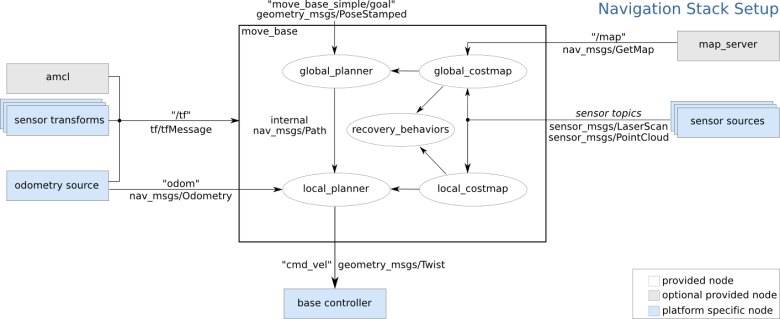
\includegraphics[width=\linewidth, center]{images/RobotSetup}
  \caption{RobotSetup tutorial navigation stack setup}
  \label{fig:RobotSetup tutorial navigation stack setup}
\end{figure}

%%%%%%%%%%%%%%%%%%%%%%%%%%%%%%%%%%%%%%%%%%%%%%%%%%%%%%%%%%%%%%%%%%%%%%%%%%%%%%%%
%%%%%%%%%%%%%%%%%%%%%%%%%%%%%%%%%%%%%%%%%%%%%%%%%%%%%%%%%%%%%%%%%%%%%%%%%%%%%%%%
\clearpage
\section{METHOD}
A detailed description of what was done, how, and why; using the mapping server, the SLAM nodes, installing plugins and running the pose array waypoint to find in rivz etc.

Using an appropriate sensor model (laser scanner or RGB-D camera) mounted on the create robot in Gazebo, an optimised system will preform SLAM in a robust manner. If an obstacle or object is added to the environment of the robot, it can update the map and navigate from point to point in an autonomous mode. 

%%%%%%%%%%%%%%%%%%%%%%%%%%%%%%%%%%%%%%%%%%%%%%%%%%%%%%%%%%%%%%%%%%%%%%%%%%%%%%%%

\subsection{Laser Scanner SDF}
 
%Details of the robot model with screenshots and sdf snippets (particularly for the laser scanner)

From the previous assignment the Hokuyo URG laser scanner will be used as the sensor for the navigation stack to orient and position itself in the map accordingly, in turn this helps the robot find the waypoints in the most optimal path. Below is the code snippet for the base laser for the topic to Rviz etc positioned on the create robot.

\begin{figure}[H]
  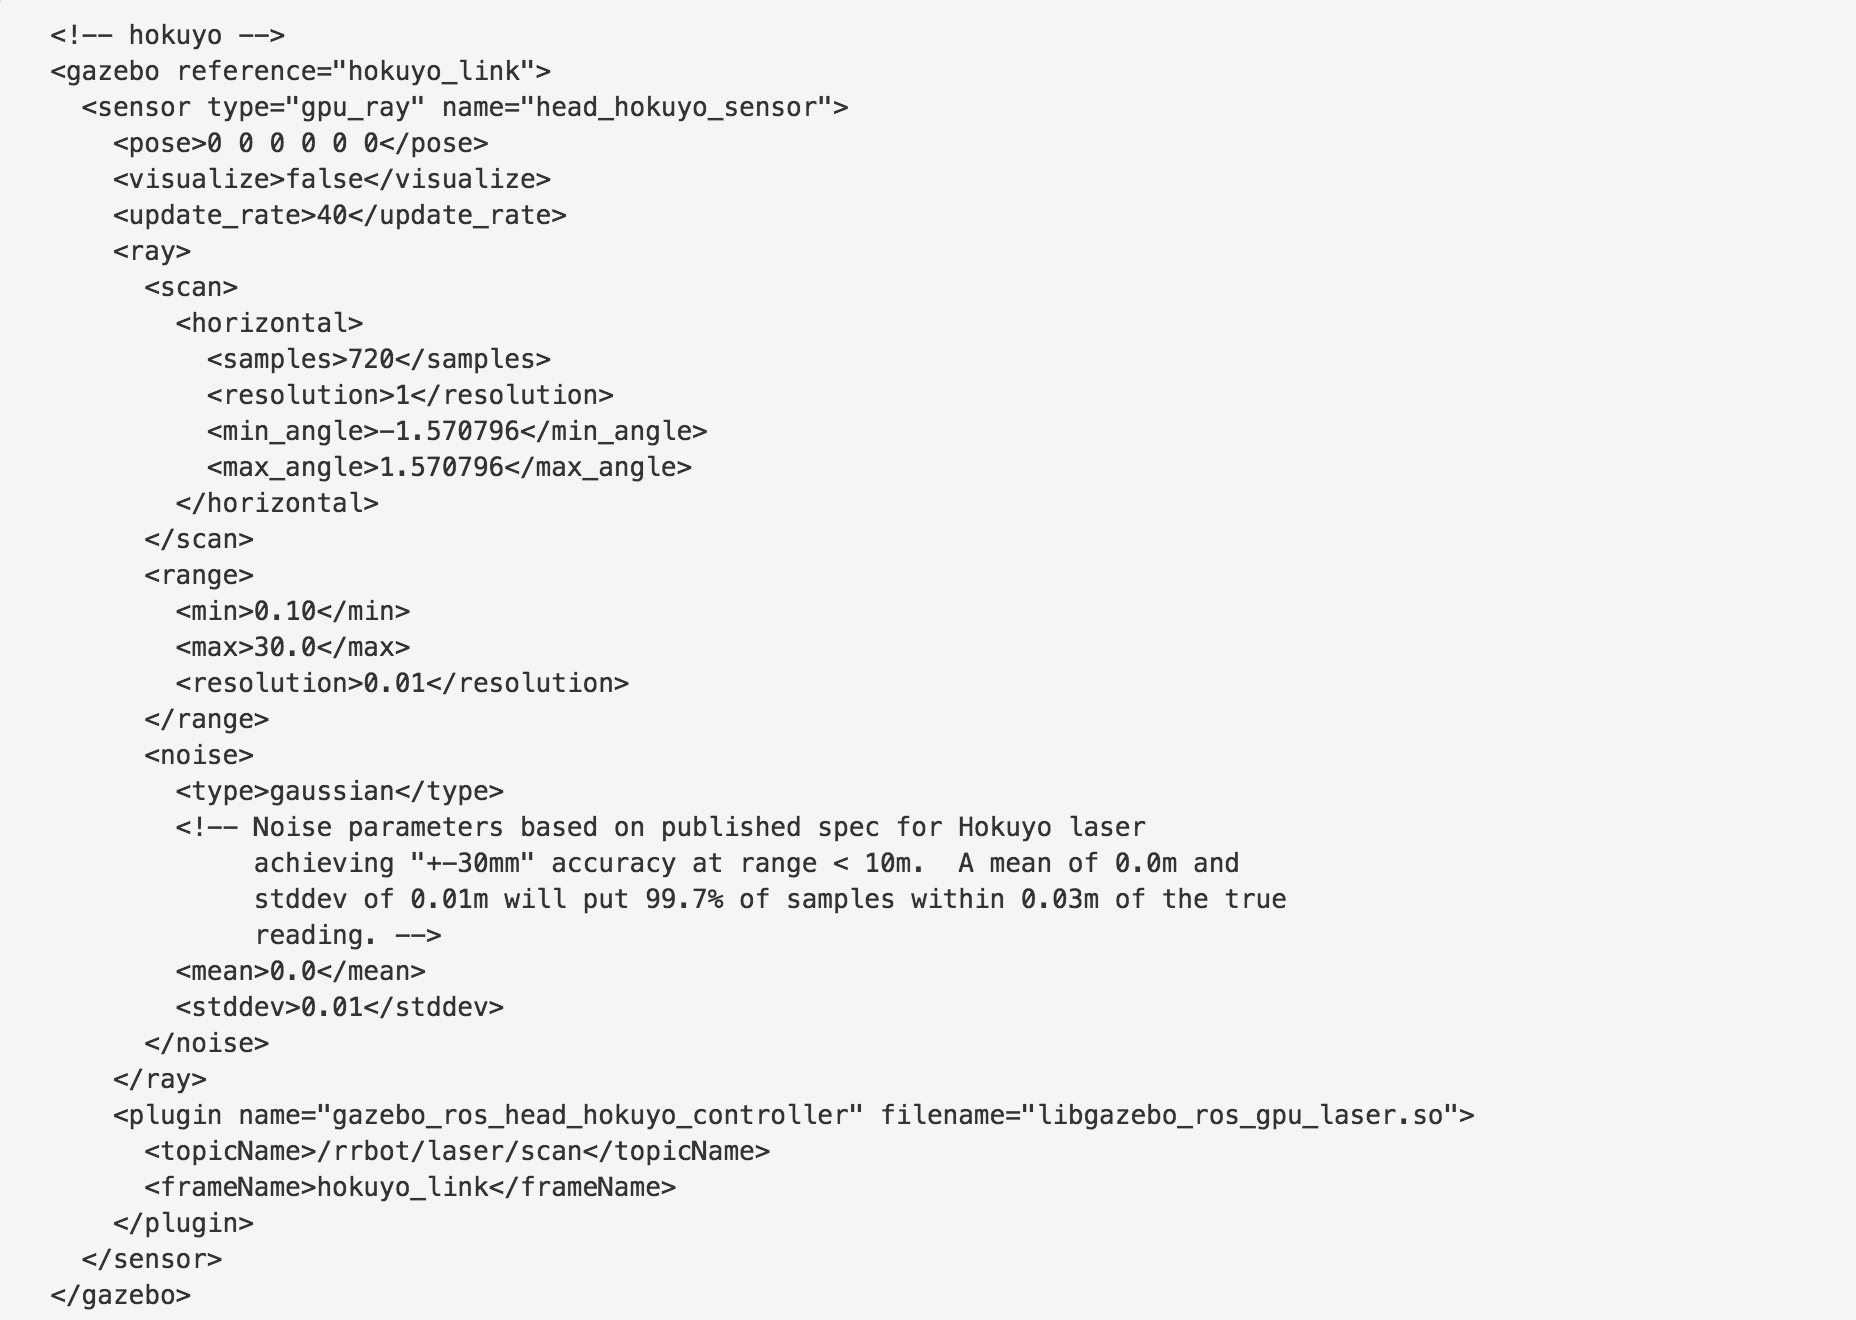
\includegraphics[width=0.7\linewidth, center]{images/laser}
  \caption{The model iRobot create sdf 1.4 version is used, the Hokuyo URG laser scanner is used}
  \label{fig:The model iRobot create sdf 1.4 version is used, the Hokuyo URG laser scanner is used}
\end{figure}

%%%%%%%%%%%%%%%%%%%%%%%%%%%%%%%%%%%%%%%%%%%%%%%%%%%%%%%%%%%%%%%%%%%%%%%%%%%%%%%%

\subsection{Pre-Requisites}

%A brief discussion on the components of navigation stack in ROS (no more than 5 pages). Append references to literature sources that describe the methods similar to those used in ROS.

In order for the 2D map to be of use, the navigation stack must be able to find the local variables and adjust accordingly. There are several pre-requisites for this to engage which include transform configurations, sensor sources(laser scanner RGB-D cam etc), odometry source, the base controller(move base), and the map server. For a more detailed explanation for the installation of these packages please refer to assignment one, and the appendix links used tutorials.

The navigation stack setup envelopes several steps of creating a package of the base, transform, odom, sensor configurations; and using the pre-configured launch file and common configurations tweaked for local and global costmap, base planner, the navigation stack is then setup and ready to be launched. Please see RobotSetup ROS tutorial link in the references for more details.

Before starting the navigation stack however, waypoints will need to be setup to act as goals to send to the navigation stack. Follow waypoints package is installed, with this package the navigation stack now has access to a new node of follow waypoint, that can passes the move base action and will subscribe and publish the Pose waypoints topics to then be set as goals for the navigation stack.

Rviz is used to then send the waypoint positions to the node and once all is set the path ready parameter is initialised. Below is an example of the waypoints in use with the navigation stack. The waypoints package used was made by Daniel Snider and is available on GitHub via the package summary link from the follow waypoints tutorial. 

\begin{figure}[H]
\begin{subfigure}[b]{0.4\textwidth}
  	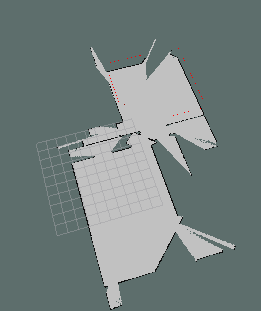
\includegraphics[width=\textwidth]{images/pgm}
  	\label{fig:using the 2D map saved to the pgm file and updated the the navigation stack from the map server the robot can show the path and position to each waypoint}
\end{subfigure}
\hfill
\begin{subfigure}[b]{0.57\textwidth}
  	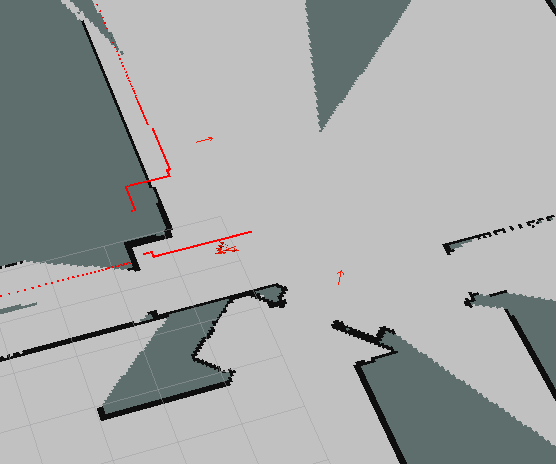
\includegraphics[width=\textwidth]{images/mapping}
  	\label{fig:Rviz showing the mapping of the robot}
\end{subfigure}
\end{figure}

Above shows using the 2D map saved to the pgm file and updated the the navigation stack from the map server the robot can show the path and position to each waypoint, Rviz showing the mapping of the robot. Now the map is successfully registering and passing to the stack the waypoints can be added. The laser sensor is shown with the red lines along the walls, with the odom as red arrows on the model and waypoints shown in pink as individual smaller arrows.


%%%%%%%%%%%%%%%%%%%%%%%%%%%%%%%%%%%%%%%%%%%%%%%%%%%%%%%%%%%%%%%%%%%%%%%%%%%%%%%%
\clearpage
\subsection{Navigation and Waypoints (Plugins)}

%Create a ROS catkin package to move the robot using move_base and gmapping. The robot should be able to navigate to goal points provided by the user in the map (in rviz). This package can be a modified version of code taken from repositories or websites but you will need to cleanly adopt it to your needs and show your contribution clearly. 

Before we begin using SLAM and Gmapping with waypoints there are several packages that need to be created and installed; these include navigations, slam gmapping, map server, follow waypoints, and other transform and base packages for odomerty and sensory etc. Once the plugins are setup as described above and are in place the robot is then ready to navigate to goal points positioned form the pose array. Please see the gmapping and RobotSetup tutorial links for the ROS website for step by step setup.

\begin{figure}[H]
\begin{subfigure}[b]{0.45\textwidth}
  	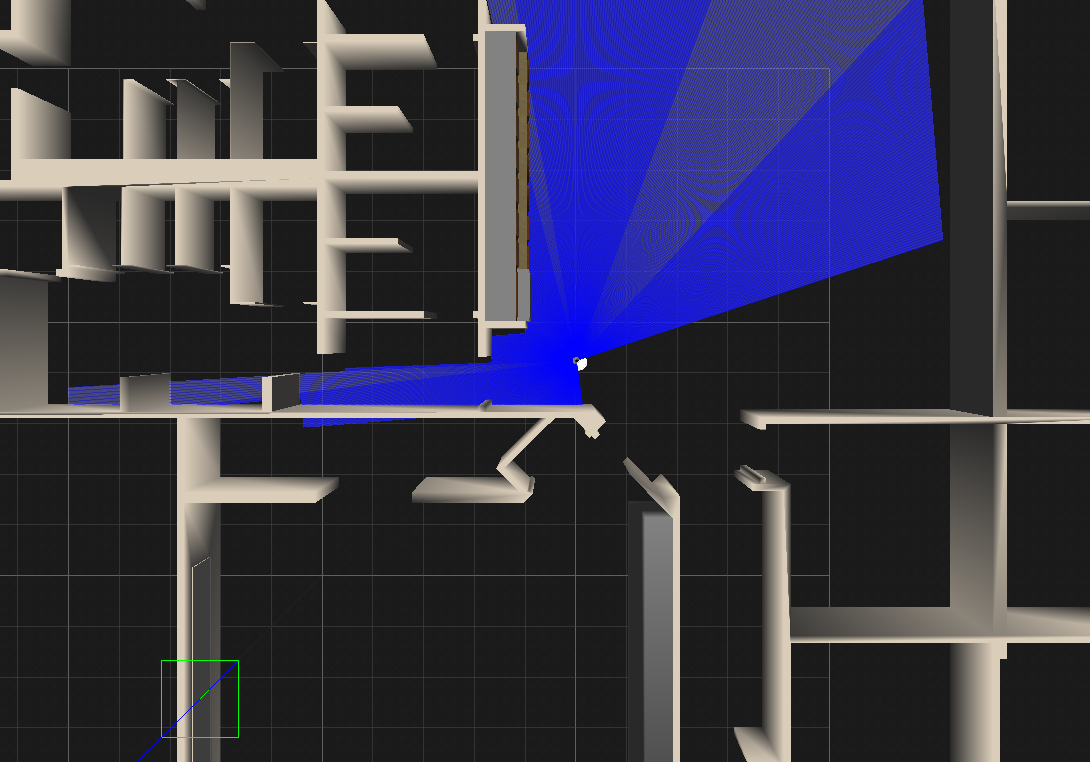
\includegraphics[width=\textwidth]{images/room1}
  	\label{fig:Live view of robot moving through rooms}
\end{subfigure}
\hfill
\begin{subfigure}[b]{0.55\textwidth}
  	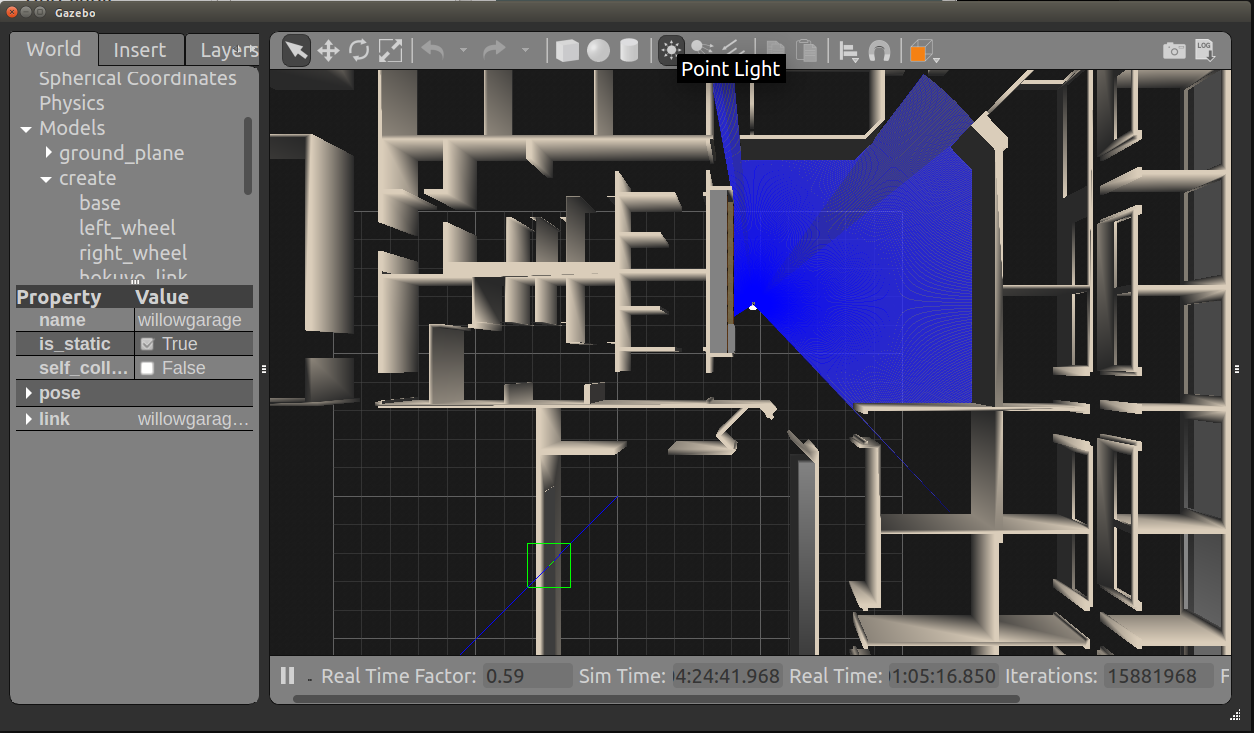
\includegraphics[width=\textwidth]{images/room2}
  	\label{fig:Robot following waypoint paths Gazebo view}
\end{subfigure}
\end{figure}

Shown above is the Gazebo graphical representation of the robot moving using SLAM to navigate using scanner attached to find a obstacles and other objects and follow the waypoints set to avoid these with the navigation stack.

Once linked the robot can begin to find itself within a local area to avoid obstacles using the navigation stack. Shown below is the demo of the first manual waypoint set and the beginning of the mapping etc.

Again Shown the rviz using the laser node with obstruction blocks and the subscribed laser topic, the representation is given by flat squares in red.

\begin{figure}[H]
  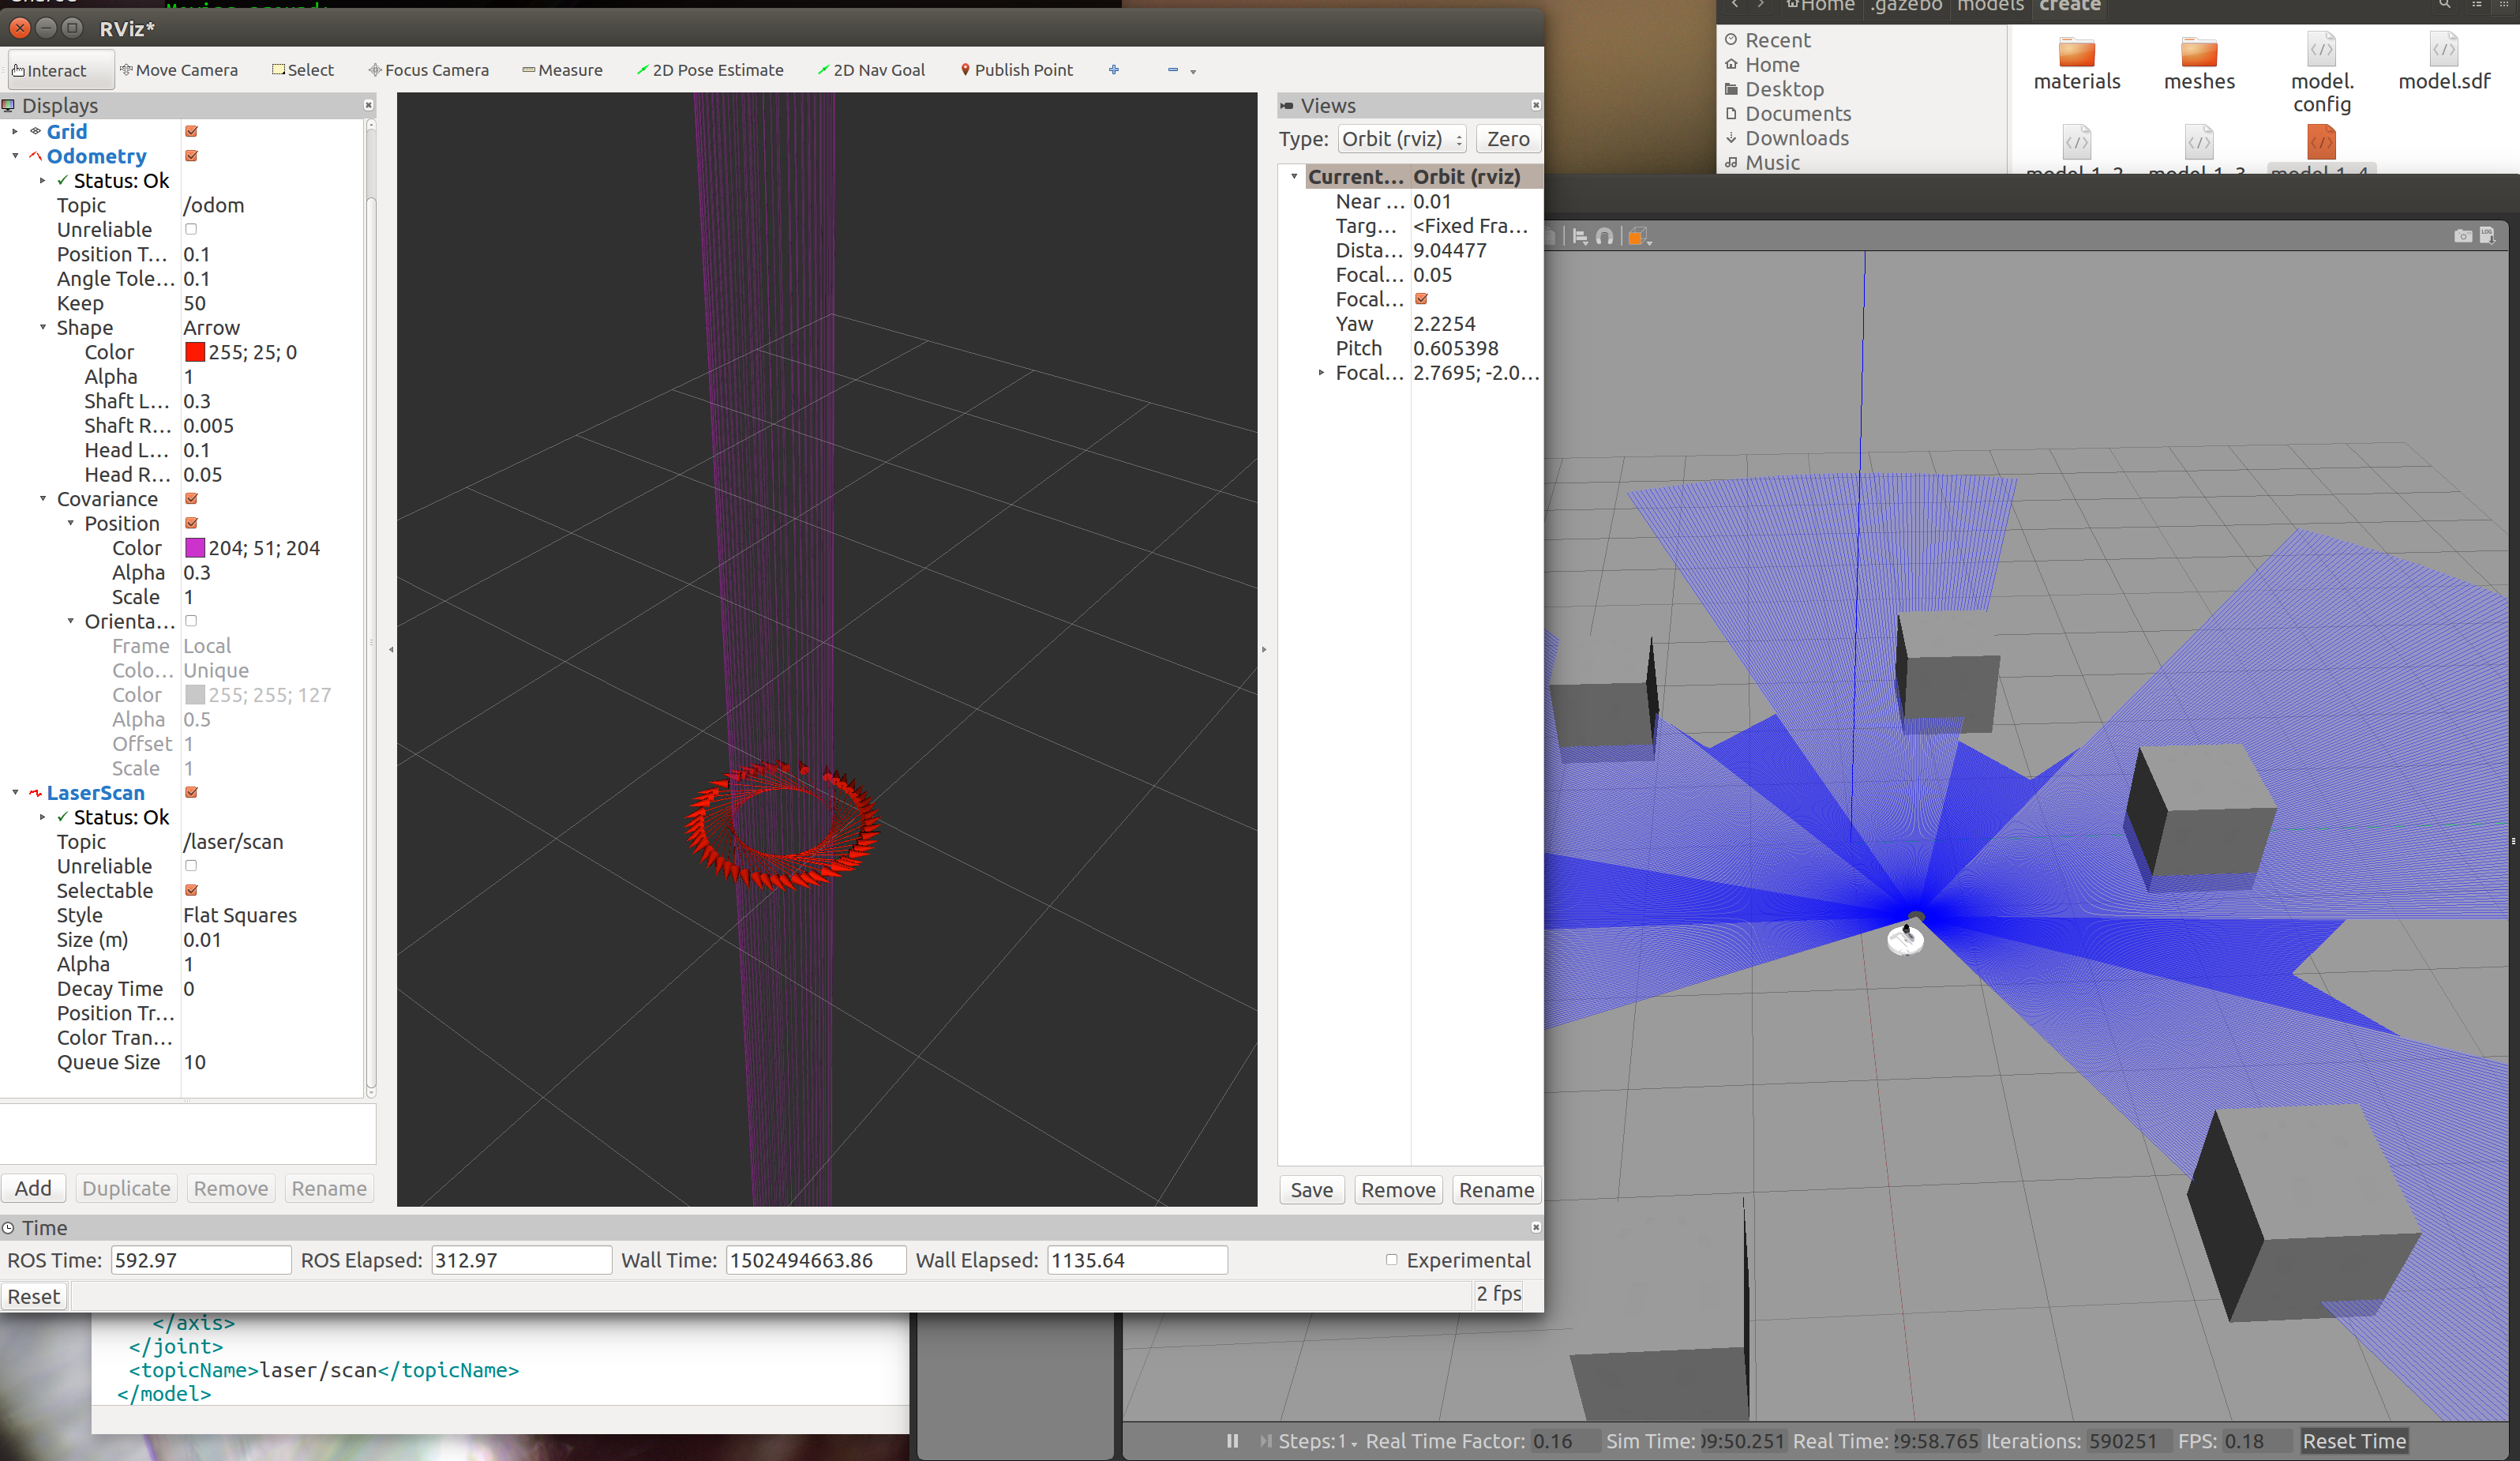
\includegraphics[width=0.8\linewidth, center]{images/rvizlaser}
  \caption{Rviz passed waypoints to the navigation stack}
  \label{fig:Rviz passed waypoints to the navigation stack}
\end{figure}

The points are provided by the user in Rviz and is passed to the navigation stack using a modified version of files from the tutorials on ROS website, please see the appendix for links and references.

\begin{figure}[H]
\begin{subfigure}{\textwidth}
	\begin{center}
  	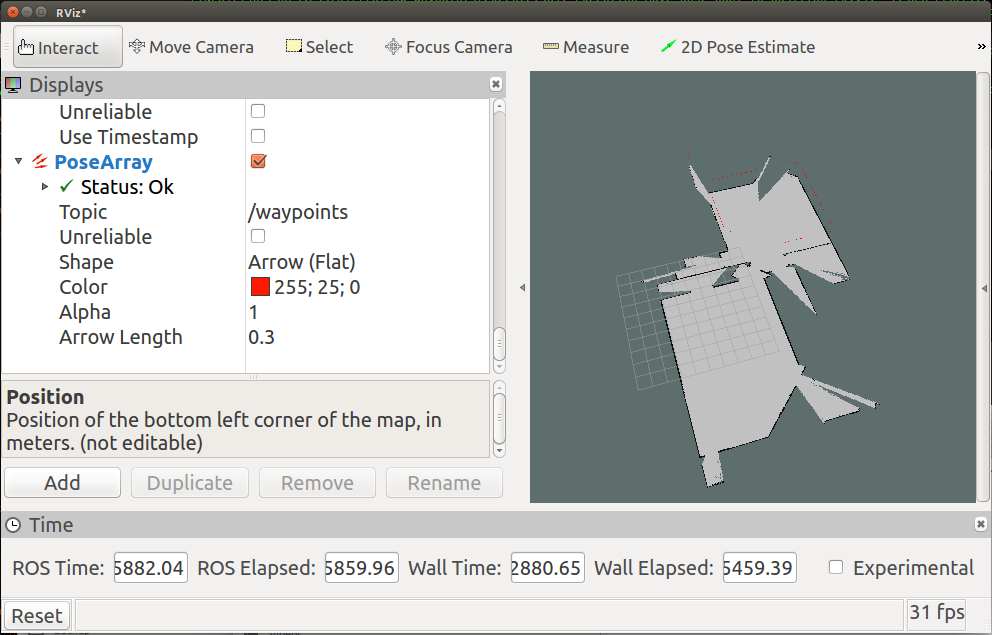
\includegraphics[width=\textwidth]{images/rviz}
  	\label{fig:Rviz setup with laser scanner showing the 2D map pgm as a live feed being saved, waypoints setup with pose array for the navigation stack}
  	\end{center}
\end{subfigure}
\begin{subfigure}{\textwidth}
	\begin{center}
  	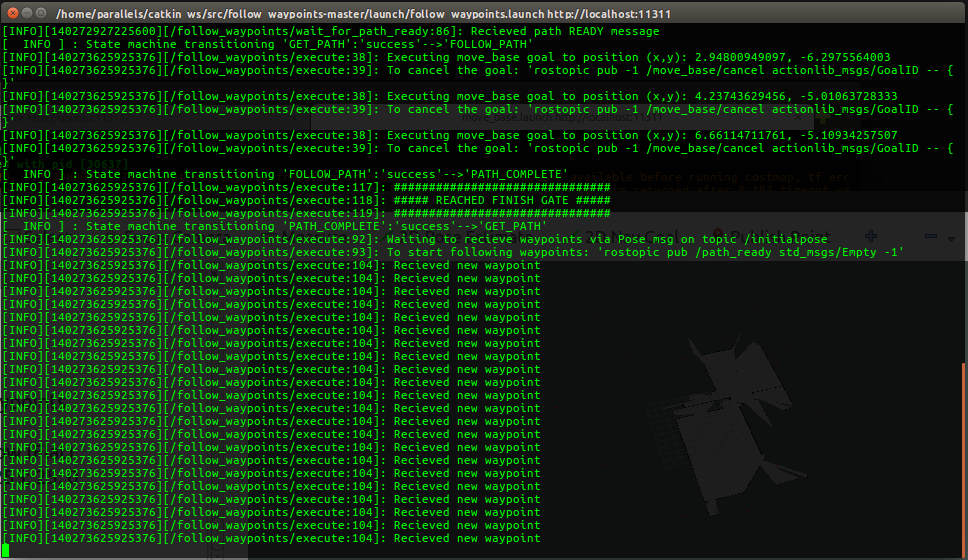
\includegraphics[width=\textwidth]{images/waypoint}
  	\label{fig:Waypoints being used with the navigation stack and the move base to goal}
  	\end{center}
\end{subfigure}
\end{figure}

After the waypoints are sent via the Pose Array the state machine will then transition and issue the Follow Path state; once the path is complete the process will then broadcast get path to say it is ready to recieve the next waypoint instruction, once they have been loaded and set the ready status can be run again to restart this process.

%%%%%%%%%%%%%%%%%%%%%%%%%%%%%%%%%%%%%%%%%%%%%%%%%%%%%%%%%%%%%%%%%%%%%%%%%%%%%%%%
\clearpage
\subsection{Pose Array Robot Control with Rviz}

%Describe important parts of your package (from #4).  

When building these packages it is important to look for areas which may require certain tuning to suit the given environment. The consideration for thresholding and inflation radius as well as min and max x speeds and such others are checked to ensure optimal performance when traveling between goals. 

While running the path there was an issue discovered with the optimal frequency which due to hardware limitations had to be manually edited to better fit the speed of the computers processing capabilities. The issue which occurred is shown below. The problem was overcome by setting the launch code frequency manually to 5hz.

\begin{figure}[H]
  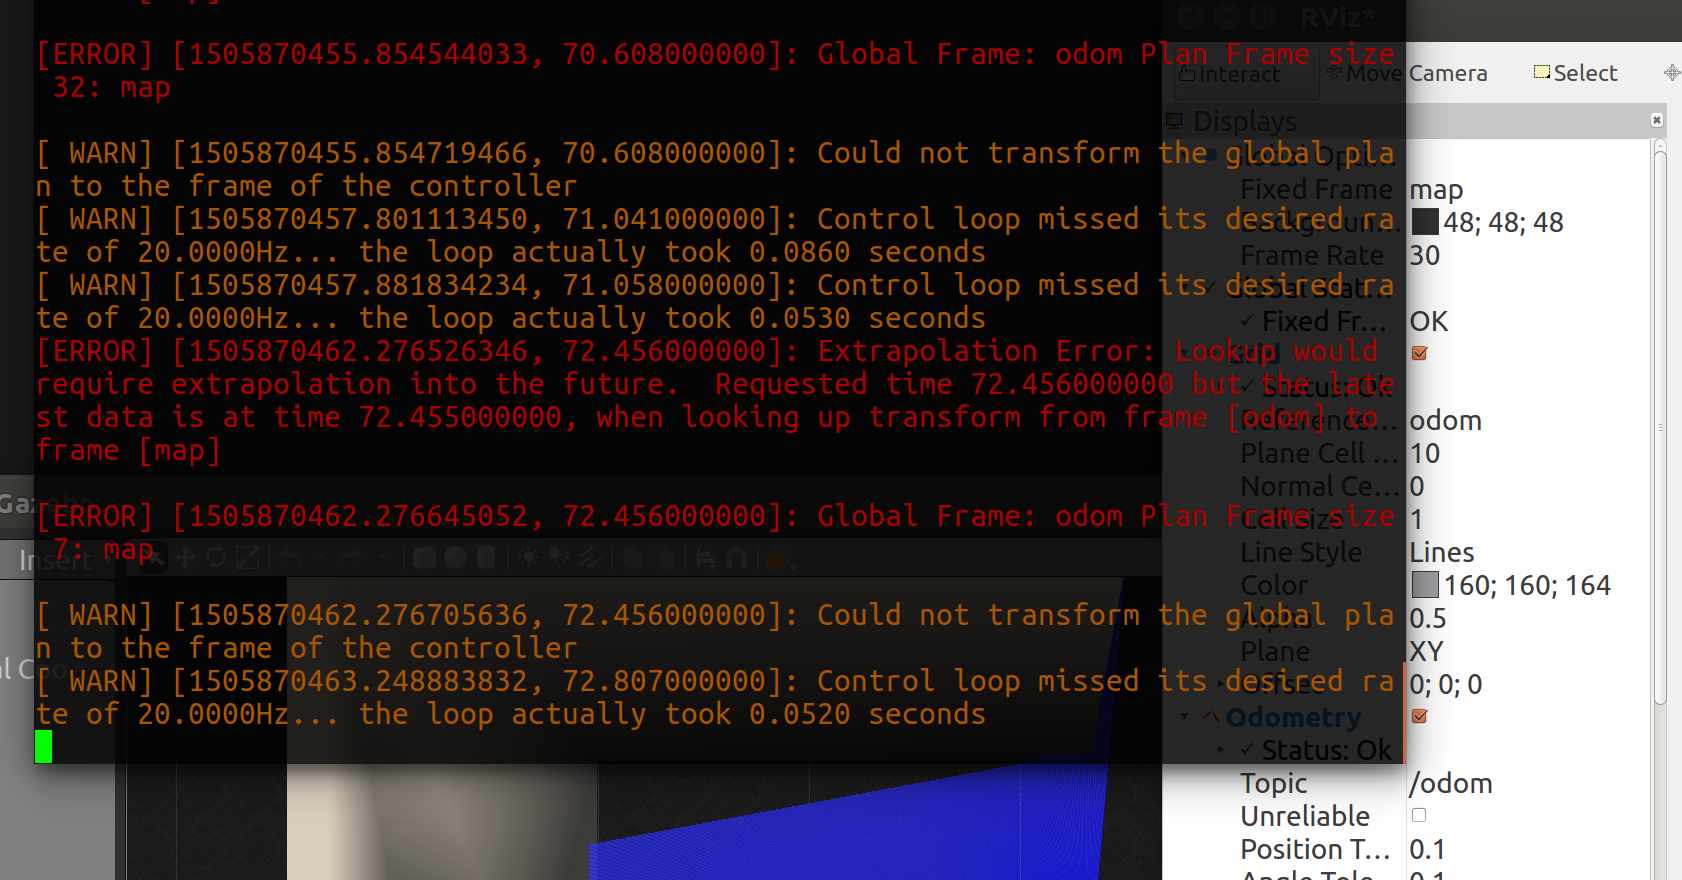
\includegraphics[width=0.8\linewidth, center]{images/error}
  \caption{Issue discovered with the optimal running frequency}
  \label{fig:Issue discovered with the optimal running frequency}
\end{figure}

After fixing all the issues and smoothing things out with trial and error tuning to find the bugs, the robot could now move freely from waypoint to waypoint as shown below

\begin{figure}[H]
  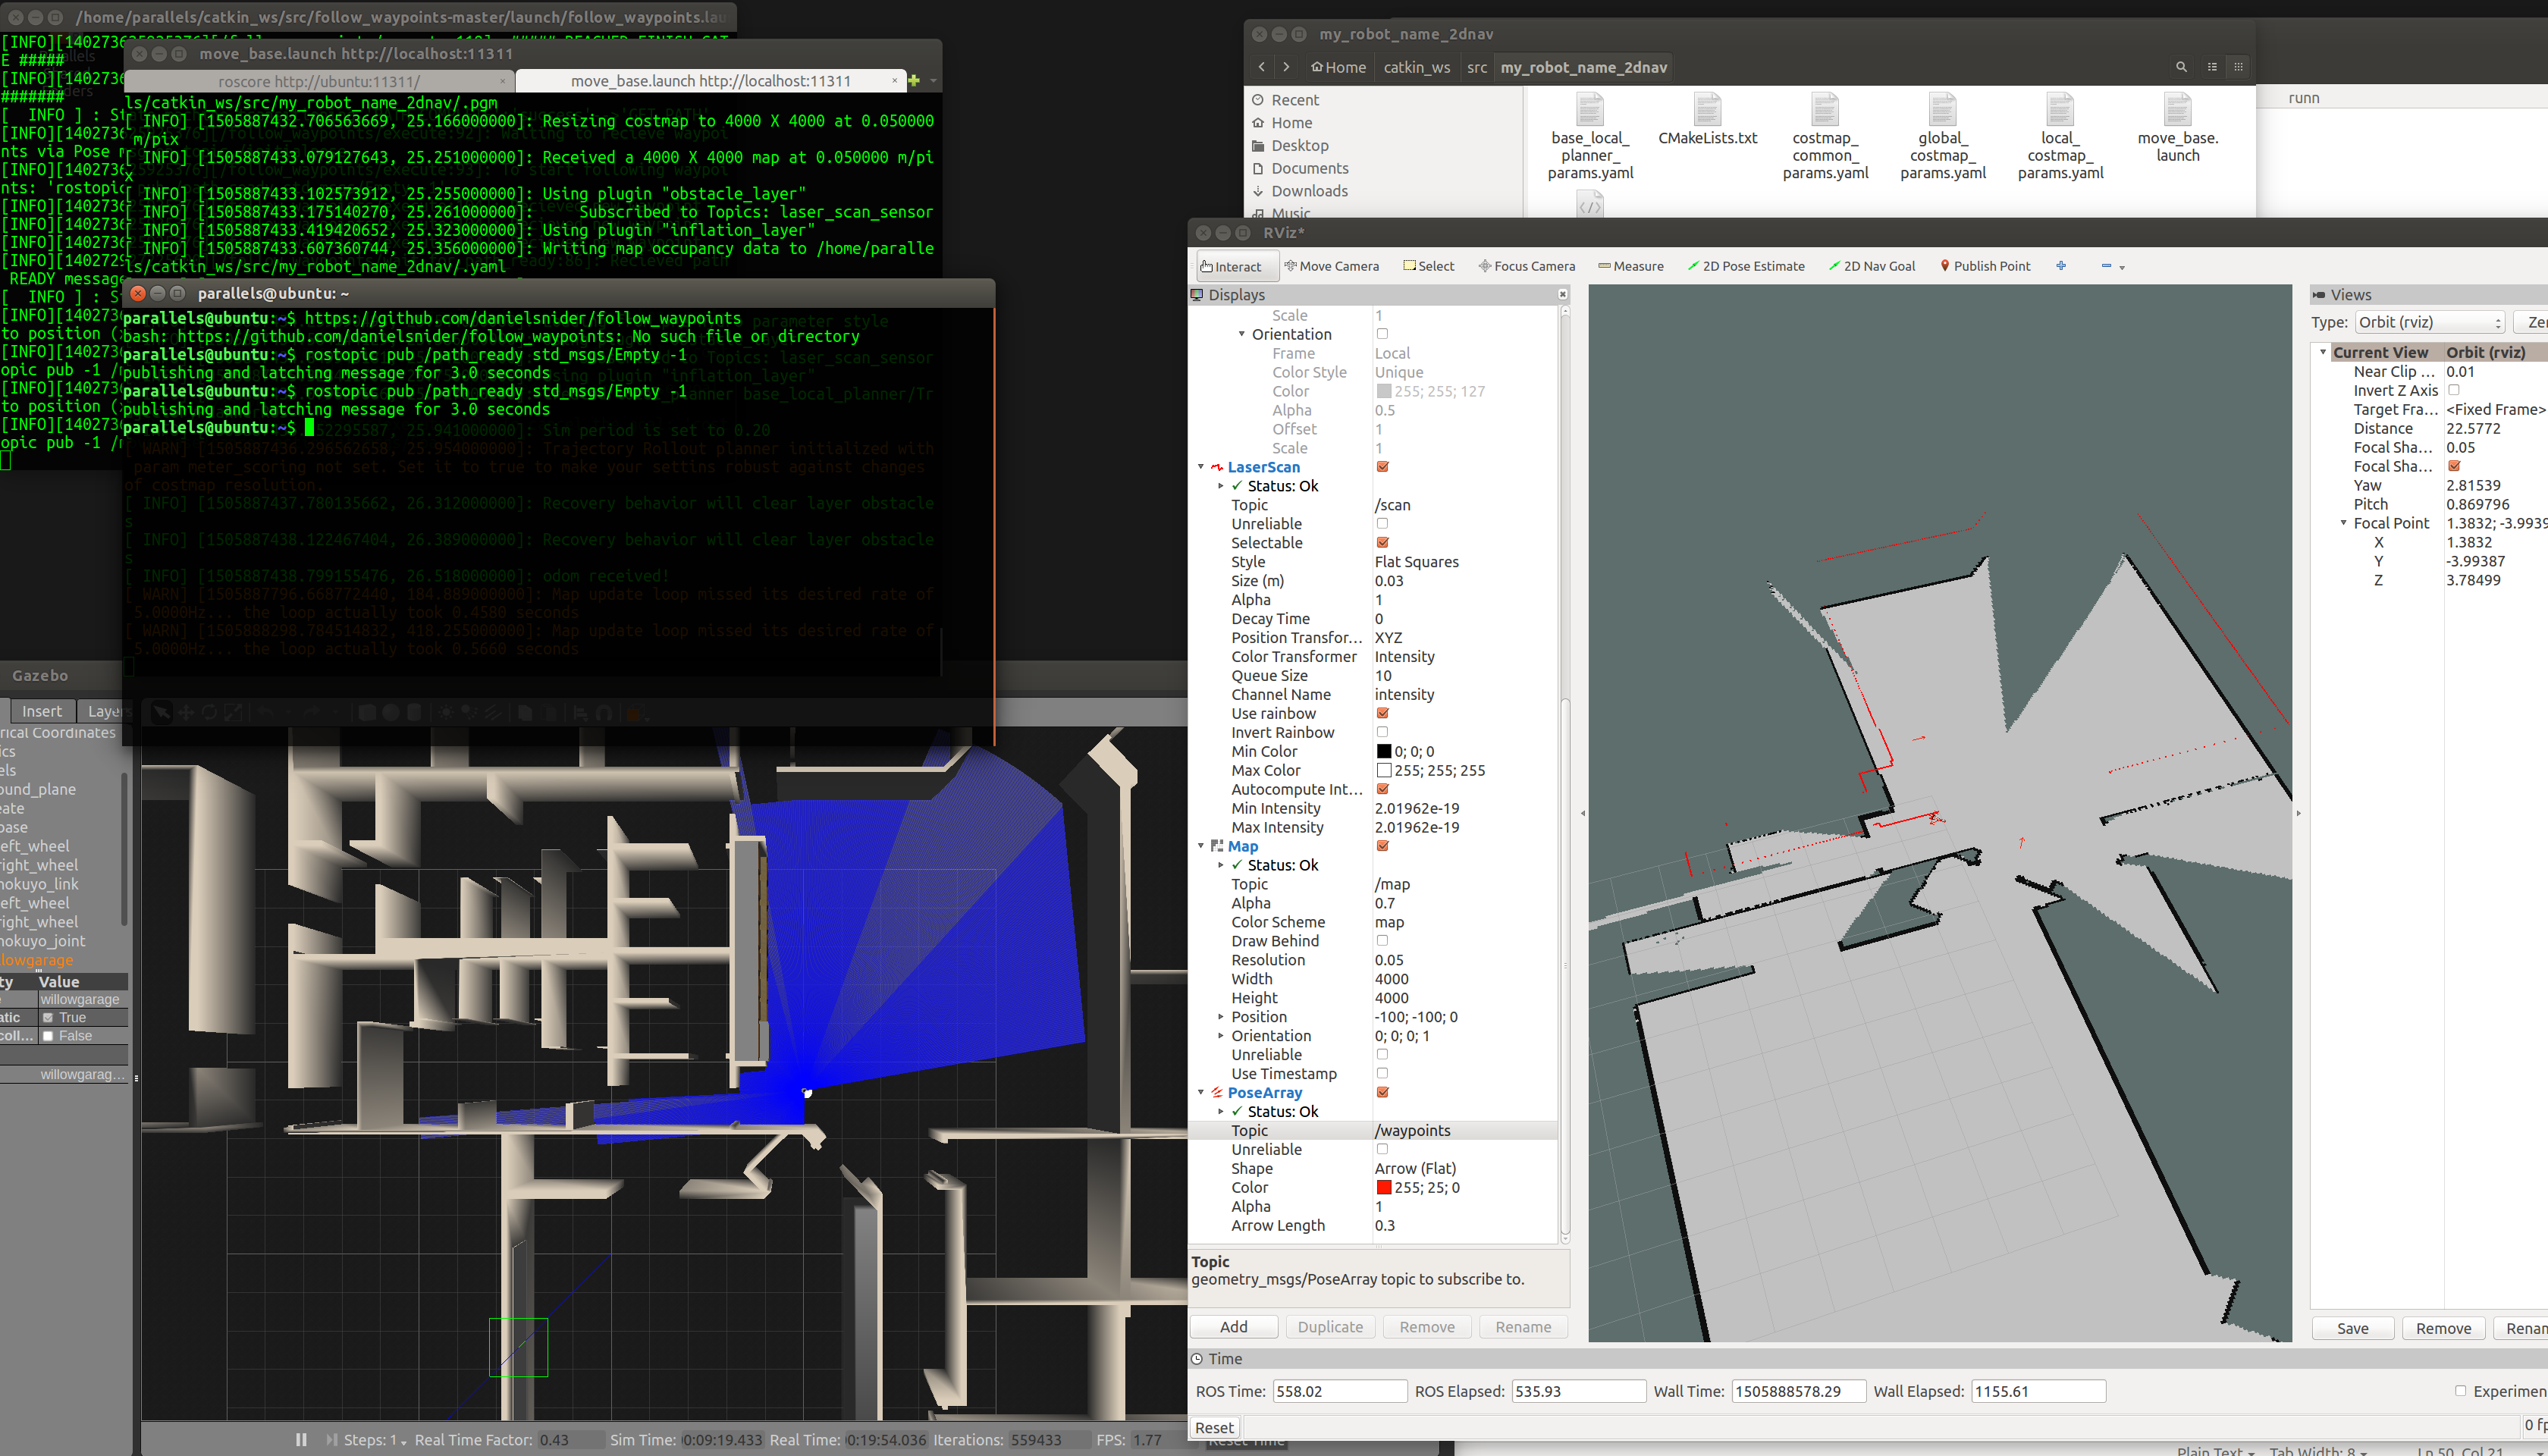
\includegraphics[width=0.8\linewidth, center]{images/total}
  \caption{Issue discovered with the optimal running frequency}
  \label{fig:Issue discovered with the optimal running frequency}
\end{figure}

%%%%%%%%%%%%%%%%%%%%%%%%%%%%%%%%%%%%%%%%%%%%%%%%%%%%%%%%%%%%%%%%%%%%%%%%%%%%%%%%

\subsection{Custom Bash Scripts}

For ease of use some bash scripts have been made to speed up the process. The scripts step through (first script "run") launching roscore, opening gazebo, importing models, creating transforms, running rviz, displaying the topic list for easy debugging, launching GMAP, launch the waypoints, and after a period of time for the points to be set to start the path. 

\begin{figure}[H]
  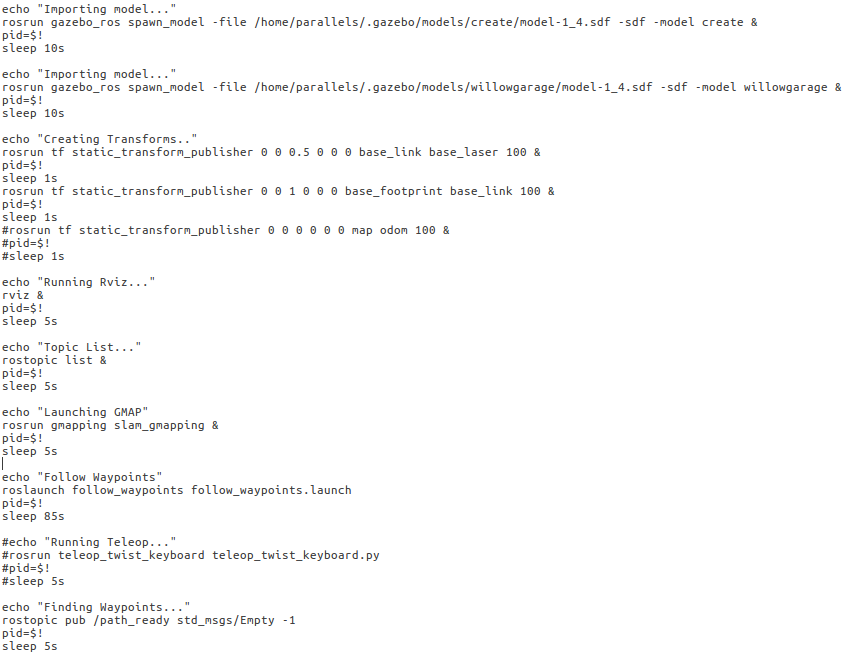
\includegraphics[width=0.8\linewidth, center]{images/run}
  \caption{"run" first bash script}
  \label{fig:"run" first bash script}
\end{figure}

While this first script is running a second script (runn) is called that starts the map server and begins updating the move base.

\begin{figure}[H]
  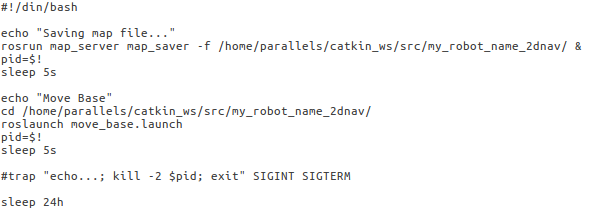
\includegraphics[width=0.8\linewidth, center]{images/runn}
  \caption{"runn" seccond bash script}
  \label{fig:"runn" seccond bash script}
\end{figure}

Once both these steps are processed the robot then begins to start the path from waypoint to waypoint and saves a pgm map as it goes detecting walls and other surrounding objects.
 
%%%%%%%%%%%%%%%%%%%%%%%%%%%%%%%%%%%%%%%%%%%%%%%%%%%%%%%%%%%%%%%%%%%%%%%%%%%%%%%%
%%%%%%%%%%%%%%%%%%%%%%%%%%%%%%%%%%%%%%%%%%%%%%%%%%%%%%%%%%%%%%%%%%%%%%%%%%%%%%%%

%\section{RESULTS}


%%%%%%%%%%%%%%%%%%%%%%%%%%%%%%%%%%%%%%%%%%%%%%%%%%%%%%%%%%%%%%%%%%%%%%%%%%%%%%%%
%%%%%%%%%%%%%%%%%%%%%%%%%%%%%%%%%%%%%%%%%%%%%%%%%%%%%%%%%%%%%%%%%%%%%%%%%%%%%%%%
\clearpage
\section{OUTCOMES}

%Submit your ROS catkin package with all necessary launch files. This code will be tested with a map and depending on the working of your robot you will get marks for this part of the report. 

Due to the size of the launch files and packages the entire workspace has been included with all relevant files and uploaded to GitHub. A Readme file has also been created to describe the contents and how to run the bash scripts for ease of use. Please note, few lines may need to be edited in the bash for the user's account, as I have used parallels virtual machine on Mac the account Home user will need to be updated accordingly etc.

Please refer to https://github.com/alex1v1a/Simulation-Modelling-and-Optimisation/tree/master/Khalid/A2 for full details and code for this assignment

Below is a full working demo shot of the create robot being used with the above mentioned navigation tasks, SLAM, the navigation stack, gampping etc

\begin{figure}[H]
  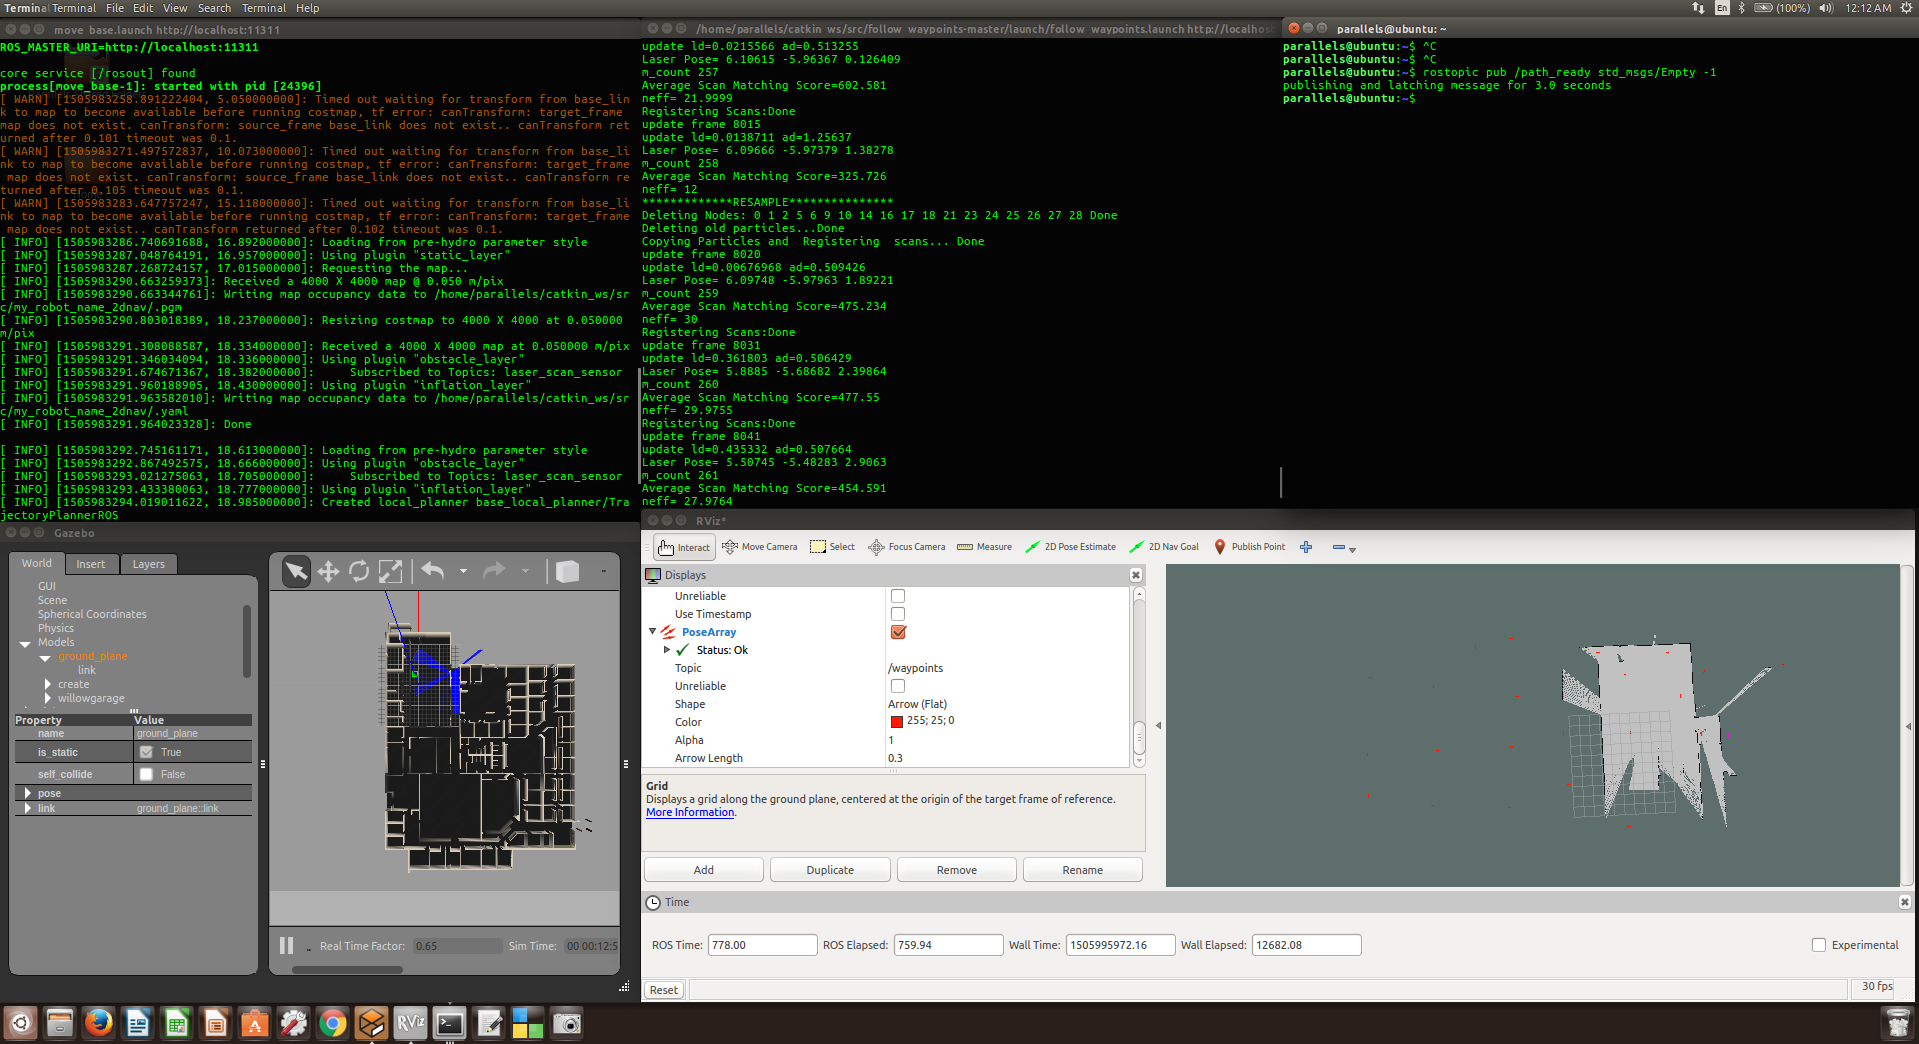
\includegraphics[width=\linewidth, center]{images/demo}
  \caption{A demo showing the full working model following waypoint goals}
  \label{fig:A demo showing the full working model following waypoint goals}
\end{figure}

The output is then displayed on the rviz graphical demonstration. A custom node is implemented to subscribe to the velocity topic and display the variable speed with a mentioned warning.


%%%%%%%%%%%%%%%%%%%%%%%%%%%%%%%%%%%%%%%%%%%%%%%%%%%%%%%%%%%%%%%%%%%%%%%%%%%%%%%%
%%%%%%%%%%%%%%%%%%%%%%%%%%%%%%%%%%%%%%%%%%%%%%%%%%%%%%%%%%%%%%%%%%%%%%%%%%%%%%%%

\section{CONCLUSIONS}

For any progress related to the report please see the public Github repo for alex1v1a or use the link in the cover page to be automatically redirected to this project. The repo provides all relative project information and files relevant to the assignment under ROS, Assignment 2

I have come to a further understanding learned more of the fundamentals of ROS using  SLAM with gmapping to travel along guided waypoints using the navigation stack with rviz user defined waypoints (posearray).

This is a powerful tool and from the basic level of understanding is an extremely vital aspect of the mechatronics processing, it is a great skill to learn.

%%%%%%%%%%%%%%%%%%%%%%%%%%%%%%%%%%%%%%%%%%%%%%%%%%%%%%%%%%%%%%%%%%%%%%%%%%%%%%%%
%%%%%%%%%%%%%%%%%%%%%%%%%%%%%%%%%%%%%%%%%%%%%%%%%%%%%%%%%%%%%%%%%%%%%%%%%%%%%%%%
\clearpage
\nocite{*}
\bibliographystyle{ieeetr}
\bibliography{references}

%%%%%%%%%%%%%%%%%%%%%%%%%%%%%%%%%%%%%%%%%%%%%%%%%%%%%%%%%%%%%%%%%%%%%%%%%%%%%%%%
%%%%%%%%%%%%%%%%%%%%%%%%%%%%%%%%%%%%%%%%%%%%%%%%%%%%%%%%%%%%%%%%%%%%%%%%%%%%%%%%

%\clearpage
%\onecolumn
%
%\section*{APPENDIX}

\end{document}
